\documentclass[border=0pt,multi,tikz]{standalone}

\usetikzlibrary{positioning}
\usetikzlibrary{patterns}
\usetikzlibrary{hobby}
\usetikzlibrary{svg.path}
\usetikzlibrary{calc}
\usetikzlibrary{decorations}
\usetikzlibrary{decorations.markings}
\usetikzlibrary{arrows.meta}
\usetikzlibrary{arrows}
\usetikzlibrary{fit}
\usetikzlibrary{fadings}

\pgfdeclarelayer{bg}    % declare background layer
\pgfsetlayers{bg,main}  % set the order of the layers (main is the standard layer)

\begin{document}
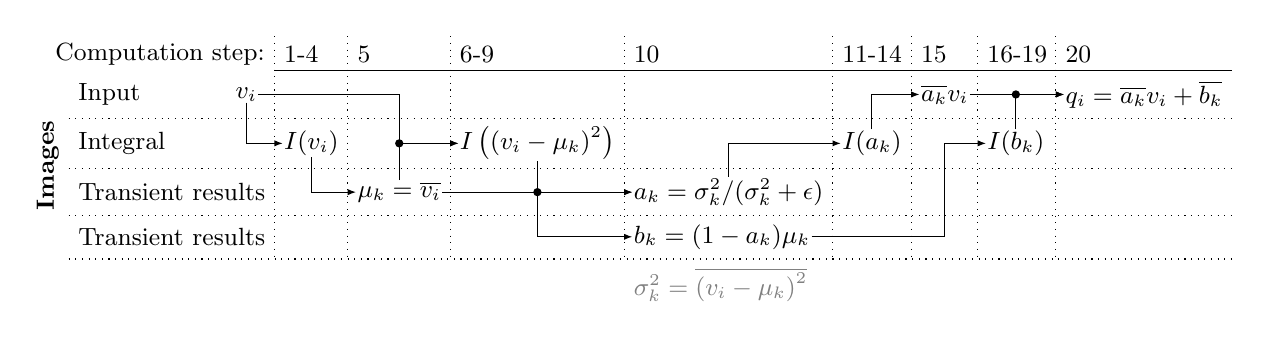
\begin{tikzpicture}[
%	xscale=1.0,
%	yscale=-0.5,
	arrow/.style={-{Latex[length=3pt]}, shorten <=-3pt, shorten >=-3pt},
	stage/.style={dotted},
	every node/.style={right,font=\small},
]

\matrix []
{
	\node(c0){}; \node(i0){}; & \node(i1){1-4}; & \node(i2){5}; & \node(i3){6-9}; & \node(i4){10}; & \node(i5){11-14}; & \node(i6){15}; & \node(i7){16-19}; & \node(i8){20}; \\
	\node(im0){Input}; & \node[](a){}; &&&&& \node(i){$\overline{a_k} v_i$}; &&  \node(k){$q_i = \overline{a_k} v_i + \overline{b_k}$}; \\
	\node(im1){Integral}; & \node(b){$I(v_i)$}; && \node(e){$I\left(\left(v_i-\mu_k\right)^2\right)$}; && \node(h){$I(a_k)$}; && \node(j){$I(b_k)$}; \\
	\node(im2){Transient results}; && \node(c){$\mu_k = \overline{v_i}$}; && \node[right](f){$a_k=\sigma_k^2 / (\sigma_k^2 + \epsilon)$}; && \\	
	\node(im3){Transient results}; &&&& \node[right](g){$b_k = (1 - a_k)\mu_k$}; \\	
    &&&& \node[gray](bot){$\sigma_k^2 = \overline{\left(v_i - \mu_k \right)^2}$}; \\
};

\node[anchor=east,xshift=-0.1cm](aa) at (a.west) {$v_i$};

\draw[arrow] (aa.south) |- (b.west);
%\draw[arrow] (a2.east) -- (b.west);
% \draw[arrow] (b.west) -- (a2.east);
\draw[arrow] (b.south) |- (c.west);
\draw[arrow] (c.east) -- (f.west);
\draw[arrow] (c.north) |- (e.west);
% \draw[arrow,ultra thick,white] (d.north) |- (e.west);
\draw[arrow] (aa.east) -| (c.south|-e.east) -- (e.west);
%\draw[arrow] (d.east) -- (e.west);
% \draw[arrow] (e.west) -- (d.east);
\draw[arrow] (e.south) |- (f.west);
\draw[arrow] (e.south) |- (g.west);
\draw[arrow] (f.north) |- (h.west);
\draw[arrow] (h.north) |- (i.west);
%\coordinate[] (is) at (g.east -| i.south);
%\draw[] (g) -- (is);
%\draw[arrow] (is) |- (j.west);
\draw[arrow] (g.east) -| (i.south|-j.west) -- (j.west);
\draw[arrow] (j.north) |- (k.west);
\draw[arrow] (i.east) -- (k.west);
\node[circle, fill=black, anchor=center,inner sep=0pt, minimum size=3pt](intersection) at (c.south|-e.east){};
\node[circle, fill=black, anchor=center,inner sep=0pt, minimum size=3pt](intersection) at (e.south|-f.west){};
\node[circle, fill=black, anchor=center,inner sep=0pt, minimum size=3pt](intersection) at (j.north|-k.west){};

\node[rotate=90,anchor=south,align=center] at ($(im0.west)!0.5!(im3.west)$) {\textbf{Images}};
\node[anchor=east,align=right] at (i1.west) {Computation step:};

% Black lines
\draw[] (i1.west|-k.north east) -- (k.north east);
% \draw[] (i0.west|-k.north east) -- (i0.south west |- bot.south);

% Dashed lines memory
\draw[stage] (im0.west|-k.south east) -- (k.south-|k.east);
\draw[stage] (im0.west|-f.north east) -- (f.north-|k.east);
\draw[stage] (im0.west|-f.south east) -- (f.south-|k.east);
\draw[stage] (im0.west|-g.south east) -- (g.south-|k.east);


% Dashed lines computation steps
\draw[stage] (i1.north west) -- (i1.west |- g.south);
\draw[stage] (i2.north west) -- (i2.west |- g.south);
\draw[stage] (i3.north west) -- (i3.west |- g.south);
\draw[stage] (i4.north west) -- (i4.west |- g.south);
\draw[stage] (i5.north west) -- (i5.west |- g.south);
\draw[stage] (i6.north west) -- (i6.west |- g.south);
\draw[stage] (i7.north west) -- (i7.west |- g.south);
\draw[stage] (i8.north west) -- (i8.west |- g.south);
%\draw[stage] (i9.north west) -- (i9.west |- bot.south);
%\draw[stage] (i10.north west) -- (i10.west |- bot.south);
\end{tikzpicture}
\end{document}